\appendix
\chapter{Statistics}
\section{Statistics - can }
% remove comment if you wish to add Appendix to contentsline.
%\addcontentsline{toc}{chapter}{Appendix A: How to download ERA5 data}
%%%% MEAN
\begin{figure}[ht]
    \centering
    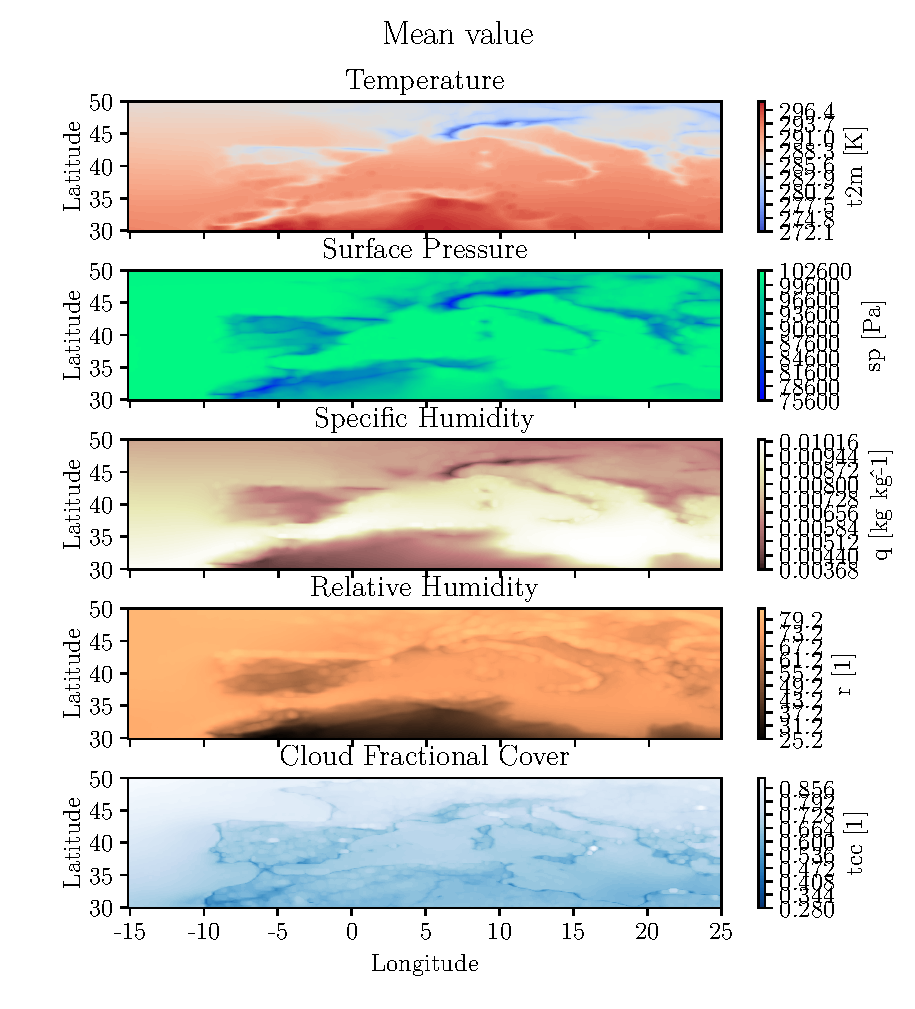
\includegraphics{python_figs/contourplot_all_variables_mean.pdf}
    \caption{Contour plot showing the local (pixel) mean of all variables.}
    \label{fig:contour_mean_all_vars}
\end{figure}




\section{Temporal statistics}

%%% ALL LOCAL STATISTICS FOR VARIABLES 
%% TEMPERATURE
\begin{figure}[ht]
    \centering
    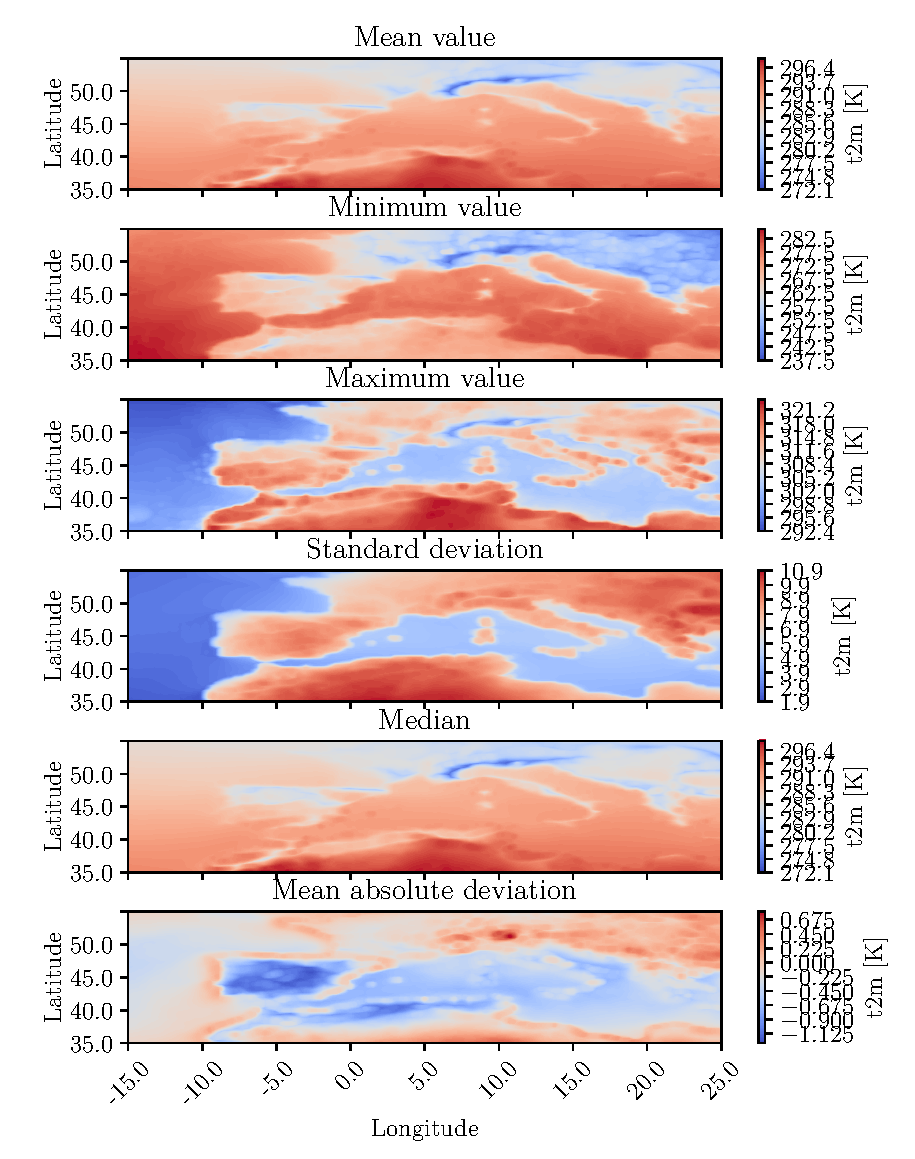
\includegraphics{python_figs/all_stat_variable_t2m.pdf}
    \caption{Contour plot showing the local (pixel) statistics for temperature.}
    \label{fig:all_stats_t2m}
\end{figure}

%% SURFACE PRESSURE 
\begin{figure}[ht]
    \centering
    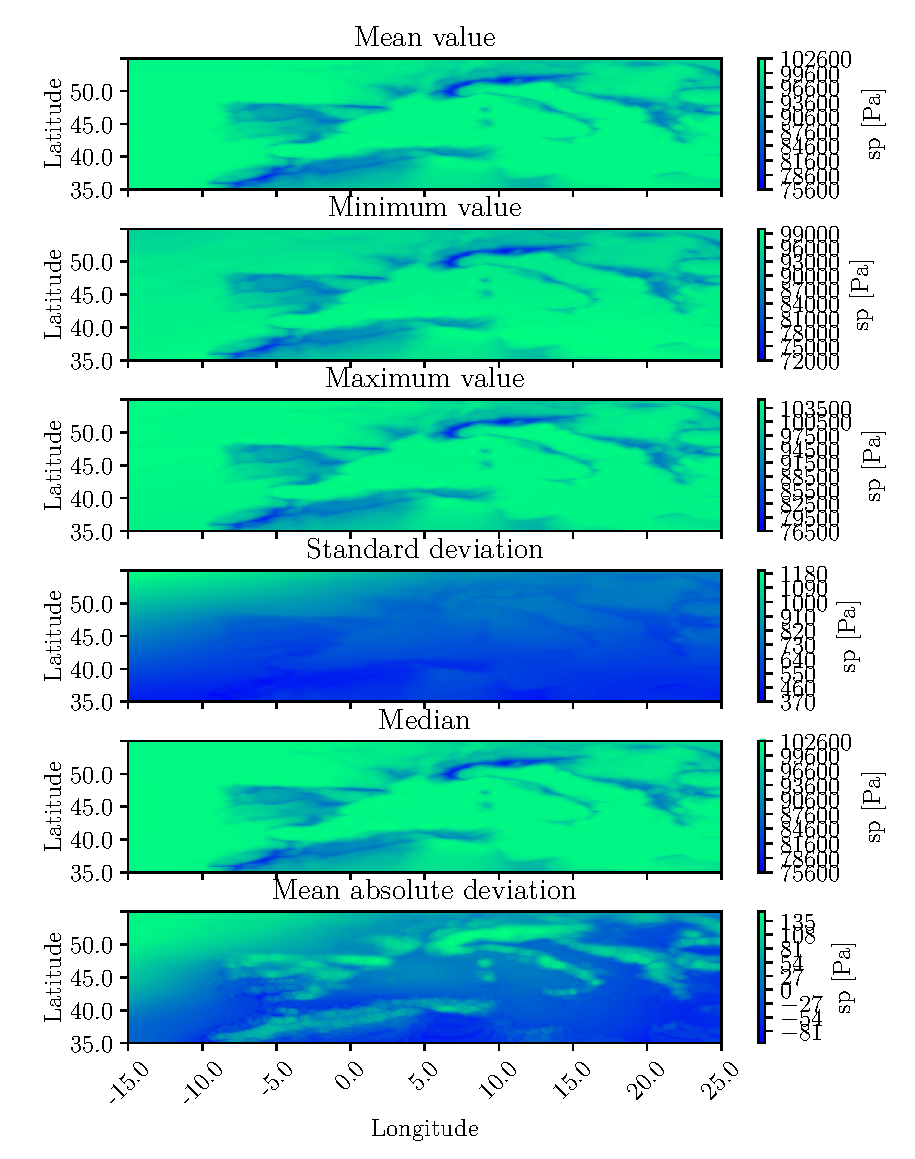
\includegraphics{python_figs/all_stat_variable_sp.pdf}
    \caption{Contour plot showing the local (pixel) statistics for surface pressure.}
    \label{fig:all_stats_sp}
\end{figure}

%% RELATIVE HUMIDITY 
\begin{figure}[ht]
    \centering
    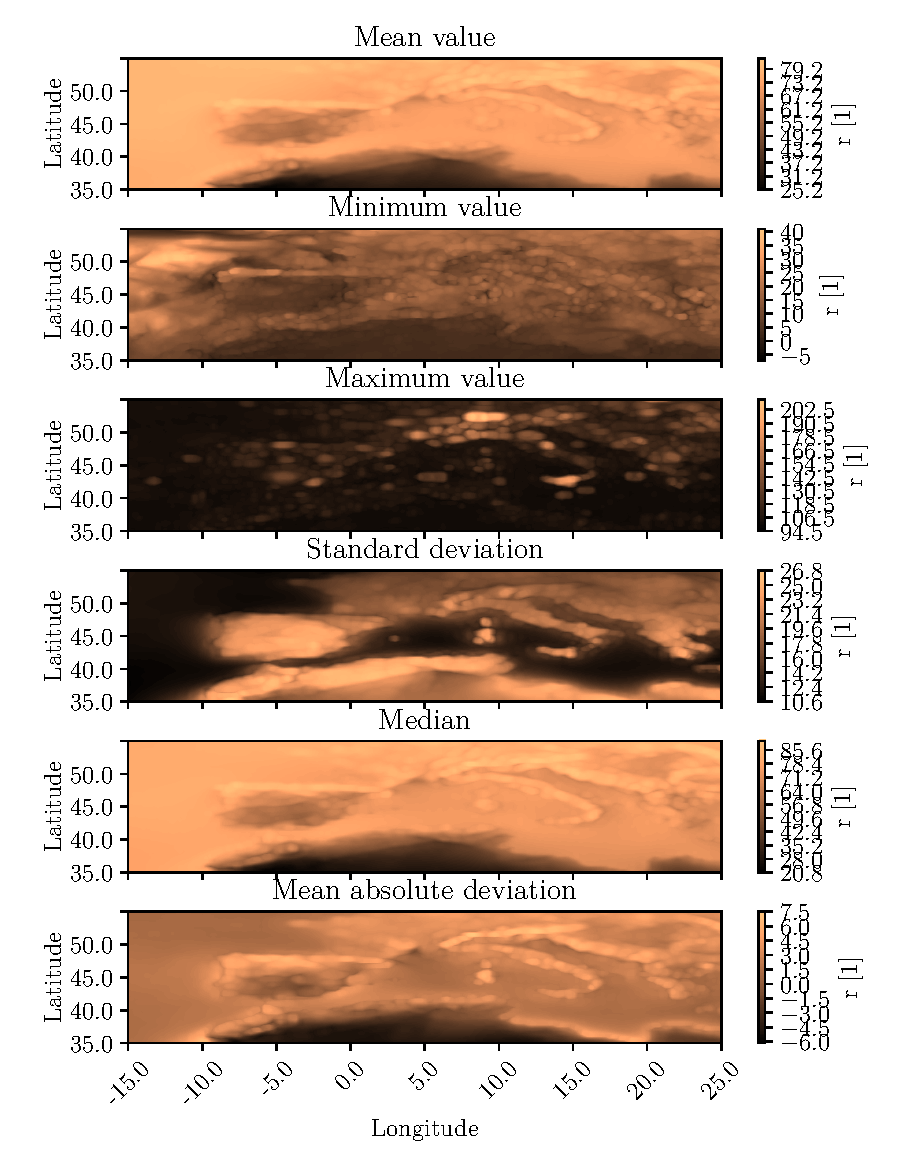
\includegraphics{python_figs/all_stat_variable_r.pdf}
    \caption{Contour plot showing the local (pixel) statistics for relative humidity.}
    \label{fig:all_stats_r}
\end{figure}


%% SPECIFIC HUMIDITY 
\begin{figure}[ht]
    \centering
    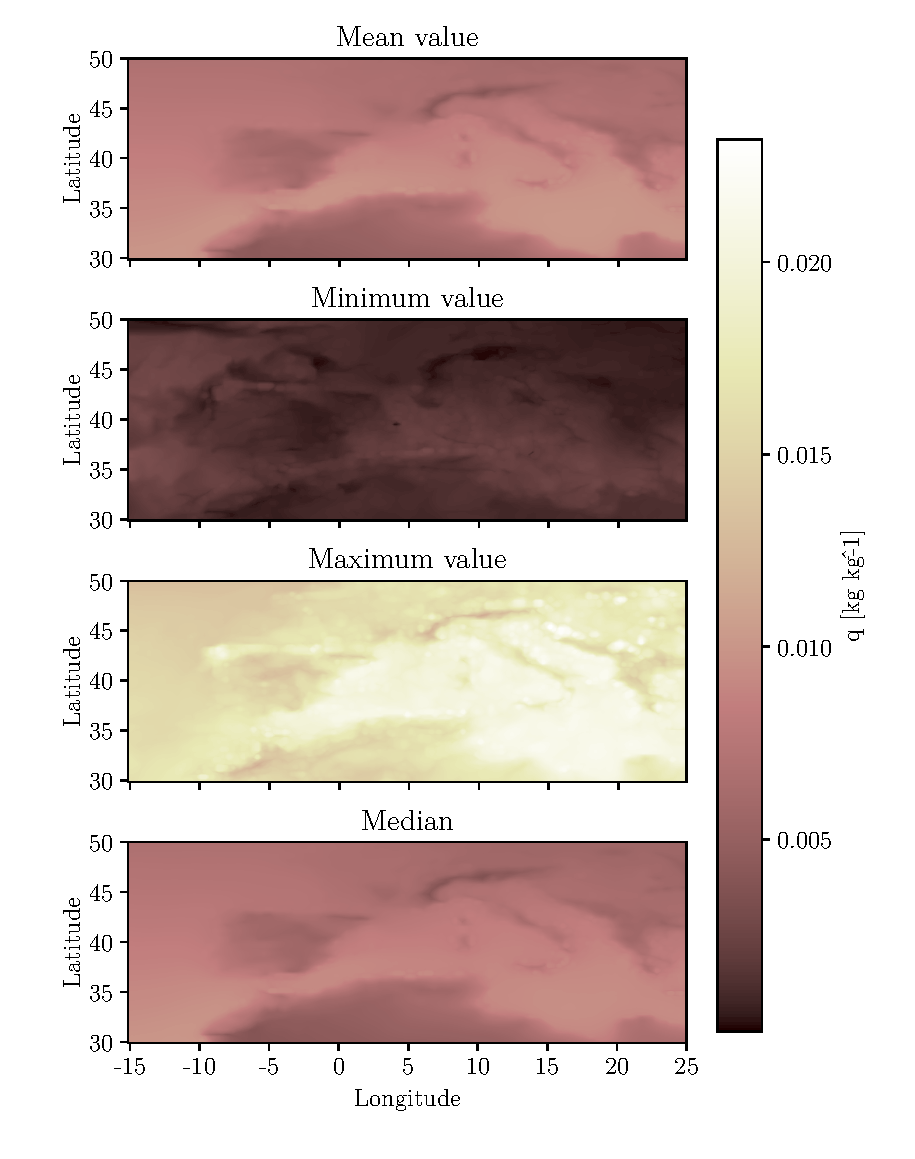
\includegraphics{python_figs/all_stat_variable_q.pdf}
    \caption{Contour plot showing the local (pixel) statistics for spesific humidity.}
    \label{fig:all_stats_q}
\end{figure}

\cleardoublepage

\chapter{Seasonal effects}
This section has more plots. 
\begin{figure}[ht]
    \centering
    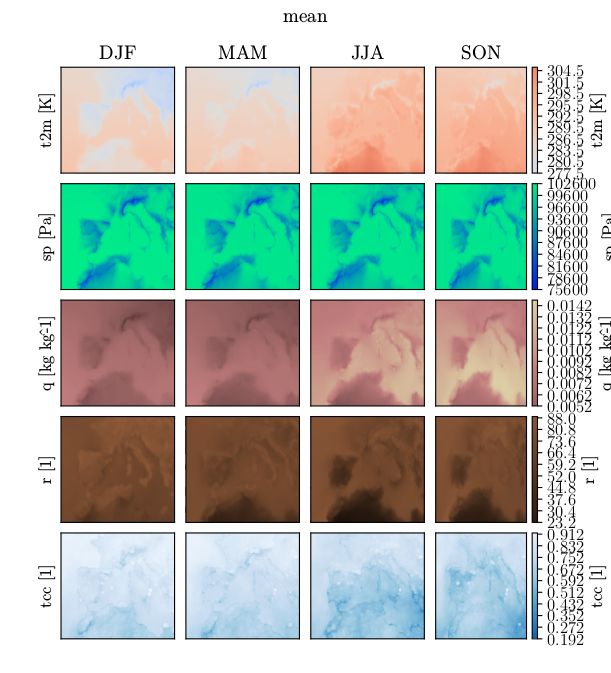
\includegraphics{python_figs/seasonal_mean_all_variables.png}
    \caption{Seasonal mean}
    \label{fig:seasonal_mean}
\end{figure}

\begin{figure}[ht]
    \centering
    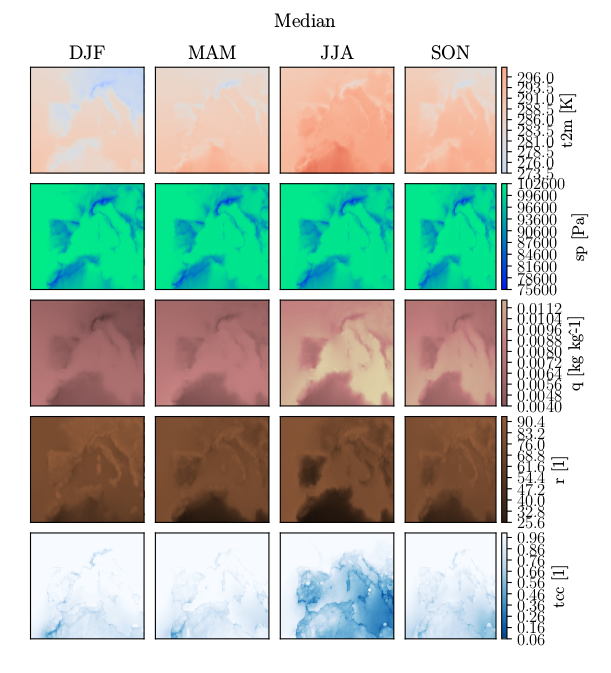
\includegraphics{python_figs/seasonal_median_all_variables.png}
    \caption{Seasonal median}
    \label{fig:seasonal_median}
\end{figure}

\chapter{Performance of other models}
Currently it show the plots that could be generated to show the performance for other model. The plots below is generated based on dummy data. 

%%%% TARGET PREDICITON HORIZONTAL
\begin{figure}[ht]
    \centering
    \includegraphics{python_figs/target_prediction_plot_horizonal.pdf}
    \caption{Comparison target and predicted cloud fractional cover.}
    \label{fig:target_predict_horizontal}
\end{figure}

%%%% TARGET PREDICITON HORIZONTAL
\begin{figure}[ht]
    \centering
    \includegraphics{python_figs/target_prediction_plot_vertical.pdf}
    \caption{Comparison target and predicted vertical cloud fractional cover.}
    \label{fig:target_predict_vertical}
\end{figure}

%%%% TARGET PREDICITON ERA5
\begin{figure}[ht]
    \centering
    \includegraphics{python_figs/target_prediction_era5_plot_horizonal.pdf}
    \caption{Comparison target, predicted and era5 horizontal cloud fractional cover.}
    \label{fig:target_predict_era5_vertical}
\end{figure}

\cleardoublepage


\chapter{Time lapse of \acrlong{tcc}}

\begin{figure}[ht]
    \centering
    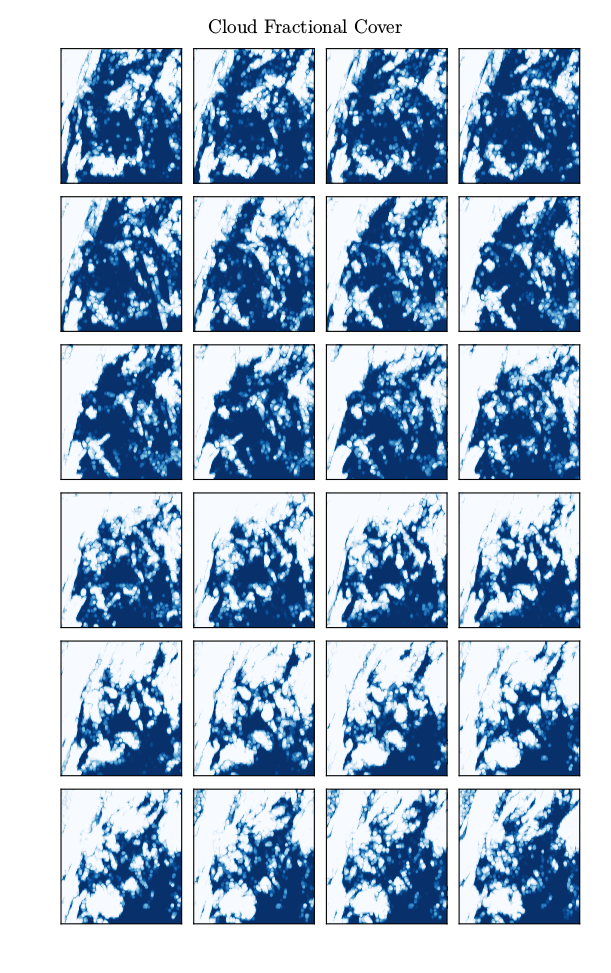
\includegraphics[scale=0.7]{python_figs/timelapse_cloud_cover_24hrs_from_2010-07-01.png}
    \caption{Time lapse photo, trying to detect the signal you would get from cloud cover within 24 hours.}
    \label{fig:time_lapse}
\end{figure}



\chapter{First week of every month in 2012}
%\addcontentsline{toc}{chapter}{Appendix D: Study 2012}

\begin{figure}[ht]
    \centering
    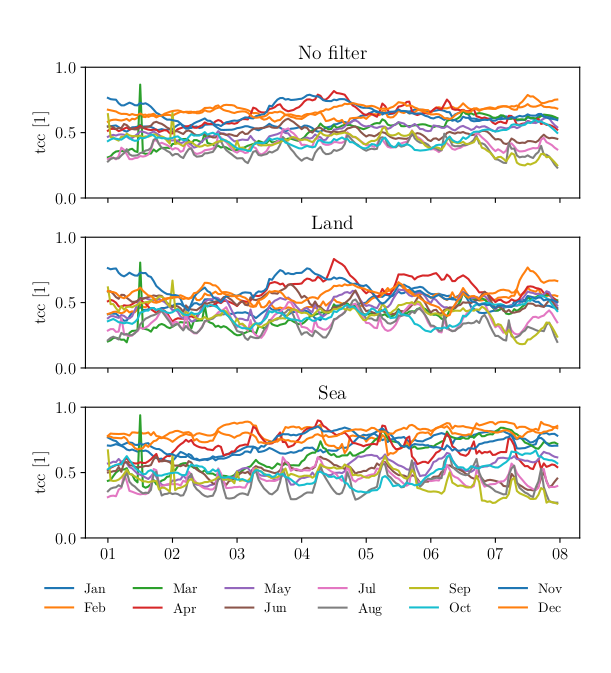
\includegraphics{python_figs/spatially_averaged_one_week_tcc_seperated_by_filters.png}
    \caption{First week of every month in 2012 merged into one figure.}
    \label{fig:all_first_week_one_figure}
\end{figure}


\begin{figure}[ht]
    \centering
    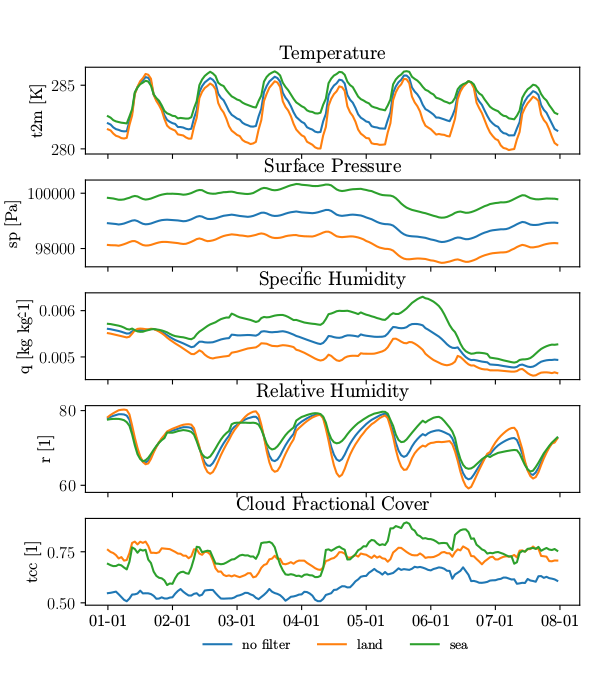
\includegraphics{python_figs/spatially_averaged_one_week_from_2012-01-01.png}
    \caption{Signal January 2012.}
    \label{fig:jan12}
\end{figure}

\begin{figure}[ht]
    \centering
    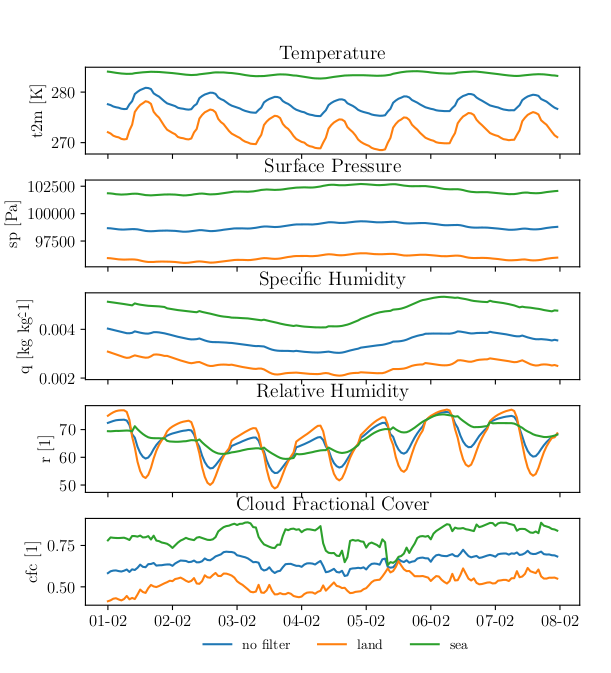
\includegraphics{python_figs/spatially_averaged_one_week_from_2012-02-01.png}
    \caption{Signal February 2012.}
    \label{fig:feb12}
\end{figure}

\begin{figure}[ht]
    \centering
    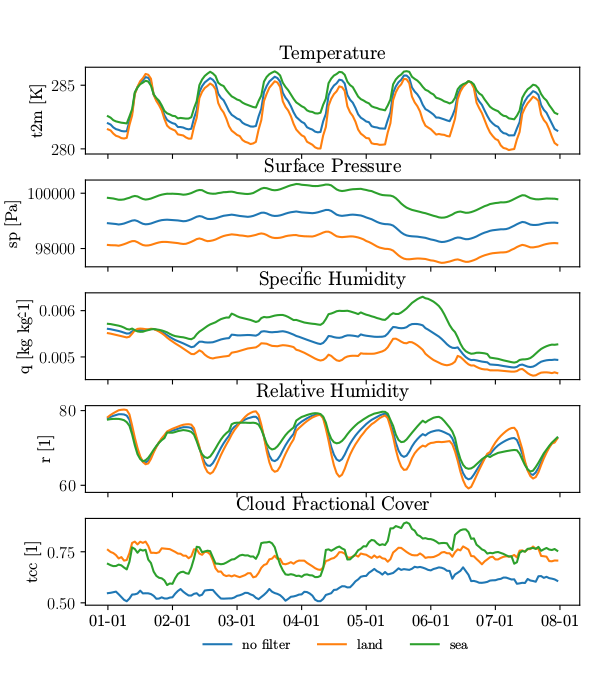
\includegraphics{python_figs/spatially_averaged_one_week_from_2012-01-01.png}
    \caption{Signal March 2012.}
    \label{fig:jan12}
\end{figure}
\begin{figure}[ht]
    \centering
    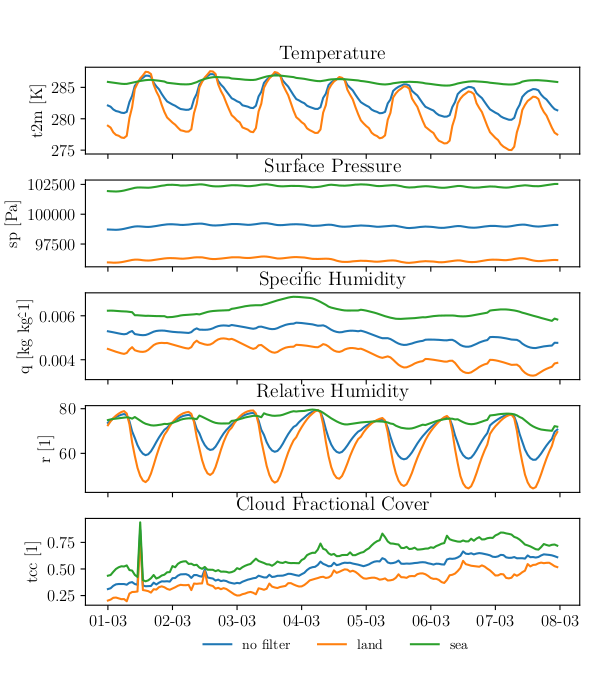
\includegraphics{python_figs/spatially_averaged_one_week_from_2012-03-01.png}
    \caption{Signal January 2012.}
    \label{fig:jan12}
\end{figure}
\begin{figure}[ht]
    \centering
    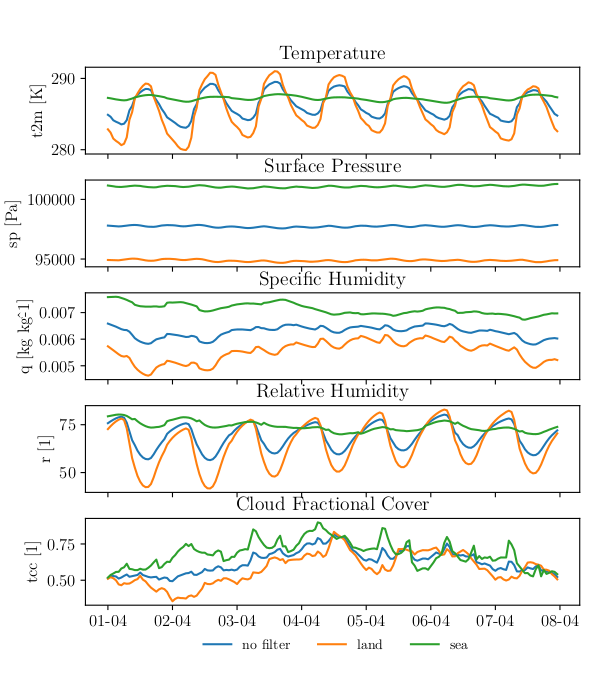
\includegraphics{python_figs/spatially_averaged_one_week_from_2012-04-01.png}
    \caption{Signal April 2012.}
    \label{fig:april12}
\end{figure}



\begin{figure}[ht]
    \centering
    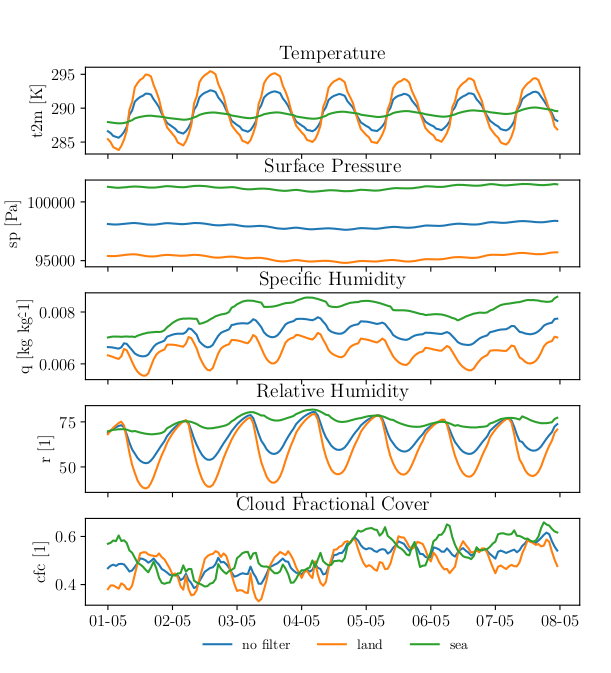
\includegraphics{python_figs/spatially_averaged_one_week_from_2012-05-01.png}
    \caption{Signal May 2012.}
    \label{fig:may12}
\end{figure}


\begin{figure}[ht]
    \centering
    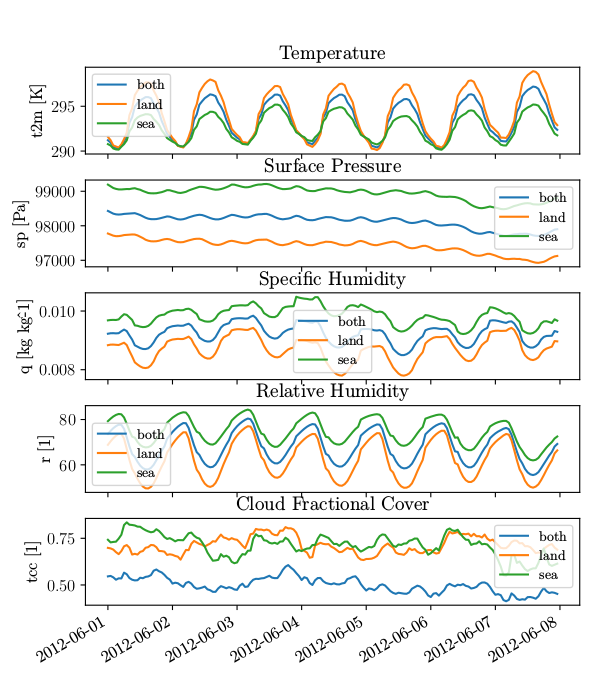
\includegraphics{python_figs/spatially_averaged_one_week_from_2012-06-01.png}
    \caption{Signal June 2012.}
    \label{fig:jun12}
\end{figure}

\begin{figure}[ht]
    \centering
    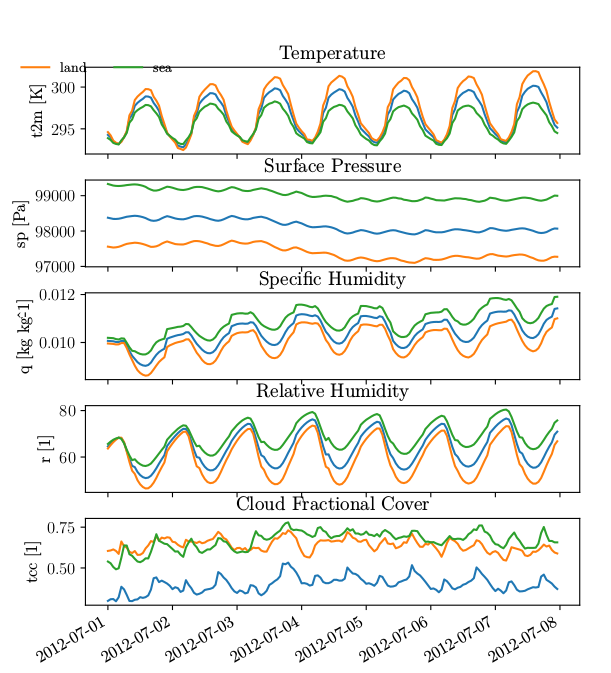
\includegraphics{python_figs/spatially_averaged_one_week_from_2012-07-01.png}
    \caption{Signal July 2012.}
    \label{fig:jul12}
\end{figure}

\begin{figure}[ht]
    \centering
    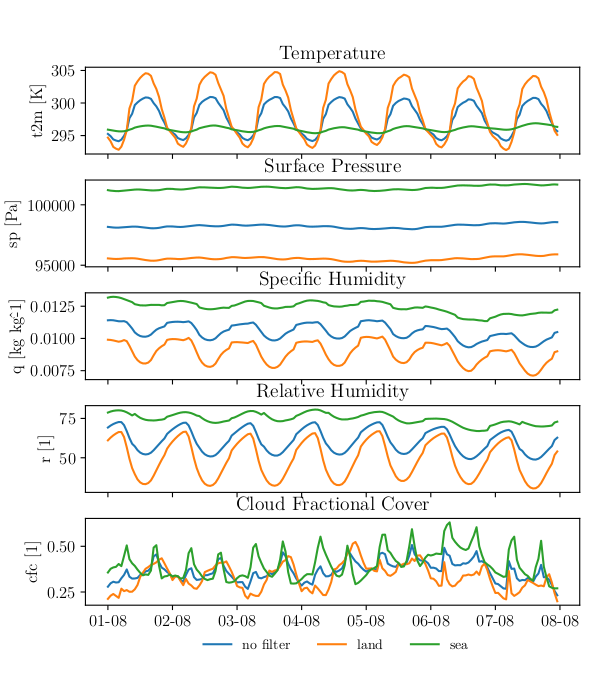
\includegraphics{python_figs/spatially_averaged_one_week_from_2012-08-01.png}
    \caption{Signal August 2012.}
    \label{fig:jan12}
\end{figure}

\begin{figure}[ht]
    \centering
    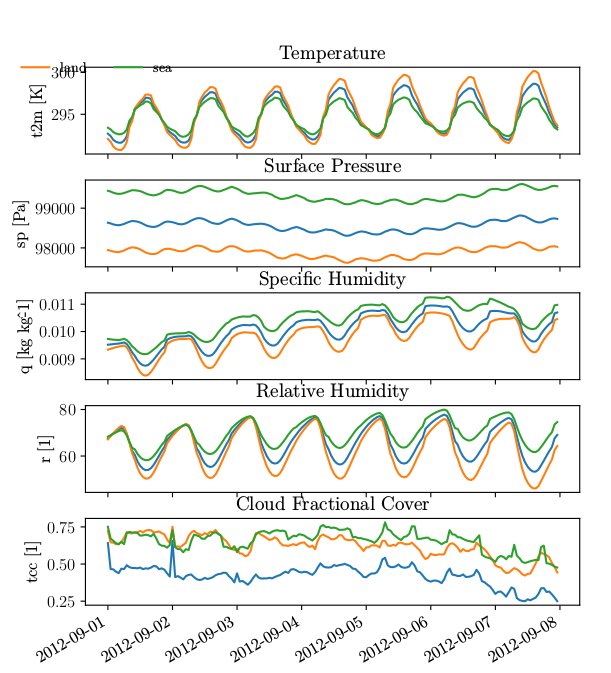
\includegraphics{python_figs/spatially_averaged_one_week_from_2012-09-01.png}
    \caption{Signal September 2012.}
    \label{fig:sep12}
\end{figure}


\begin{figure}[ht]
    \centering
    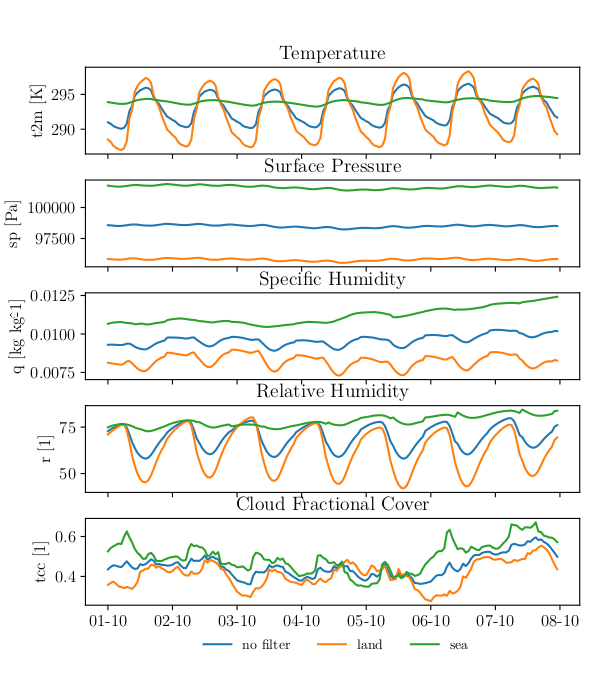
\includegraphics{python_figs/spatially_averaged_one_week_from_2012-10-01.png}
    \caption{Signal October 2012.}
    \label{fig:oct12}
\end{figure}


\begin{figure}[ht]
    \centering
    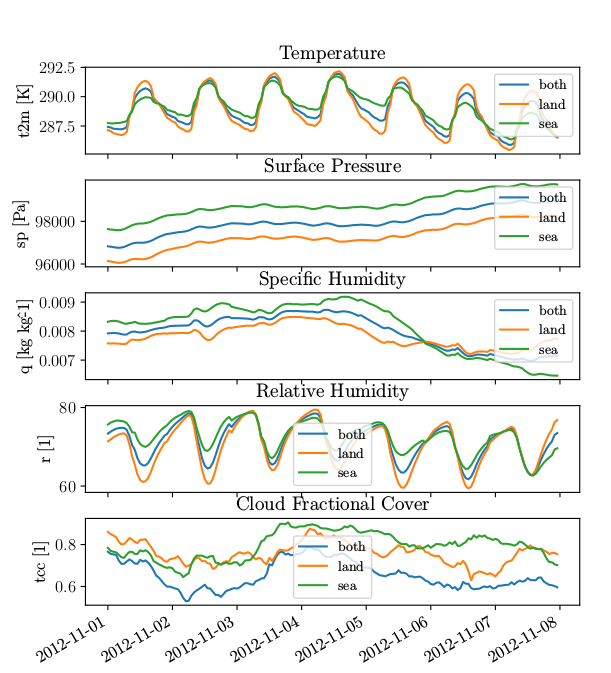
\includegraphics{python_figs/spatially_averaged_one_week_from_2012-11-01.png}
    \caption{Signal November 2012.}
    \label{fig:nov12}
\end{figure}

\begin{figure}[ht]
    \centering
    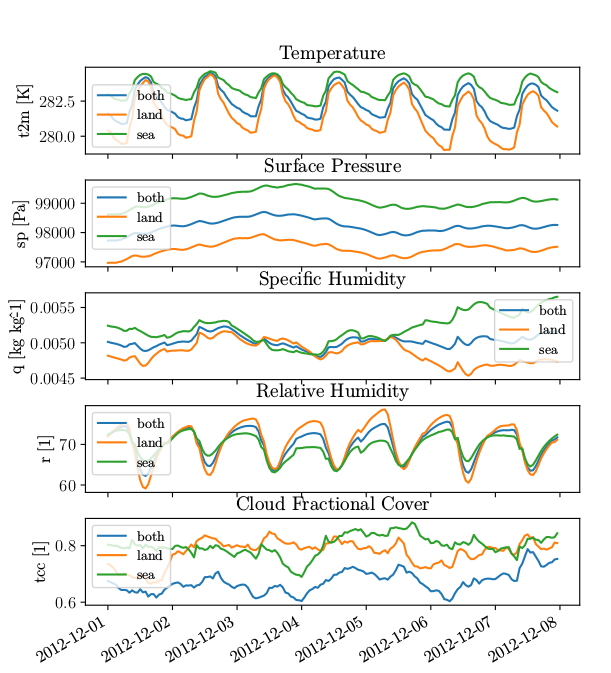
\includegraphics{python_figs/spatially_averaged_one_week_from_2012-12-01.png}
    \caption{Signal December 2012.}
    \label{fig:dec12}
\end{figure}


%%%%%%%%%%%%%%%%%%%%%%%%%%%%%%%%%%%%% signal artefact should be redefined if used 
\begin{figure}
    \centering
    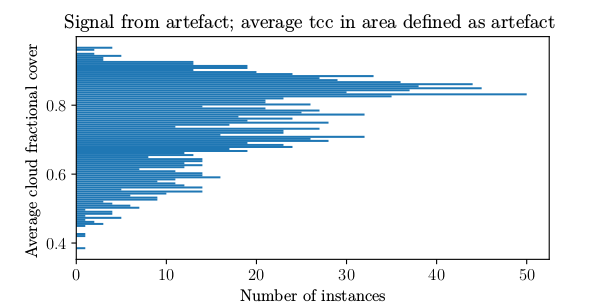
\includegraphics{python_figs/signal_artefact.png}
    \caption{Occurence of artefact, keep in mind that is not made any effort to distinguish this from when the entire area has cloud cover, this could be done by the ratio of artefact signal to land or something else. }
    \label{fig:signal_artefact}
\end{figure}
